\documentclass[twoside]{book}

% Packages required by doxygen
\usepackage{fixltx2e}
\usepackage{calc}
\usepackage{doxygen}
\usepackage[export]{adjustbox} % also loads graphicx
\usepackage{graphicx}
\usepackage[utf8]{inputenc}
\usepackage{makeidx}
\usepackage{multicol}
\usepackage{multirow}
\PassOptionsToPackage{warn}{textcomp}
\usepackage{textcomp}
\usepackage[nointegrals]{wasysym}
\usepackage[table]{xcolor}

% Font selection
\usepackage[T1]{fontenc}
\usepackage[scaled=.90]{helvet}
\usepackage{courier}
\usepackage{amssymb}
\usepackage{sectsty}
\renewcommand{\familydefault}{\sfdefault}
\allsectionsfont{%
  \fontseries{bc}\selectfont%
  \color{darkgray}%
}
\renewcommand{\DoxyLabelFont}{%
  \fontseries{bc}\selectfont%
  \color{darkgray}%
}
\newcommand{\+}{\discretionary{\mbox{\scriptsize$\hookleftarrow$}}{}{}}

% Page & text layout
\usepackage{geometry}
\geometry{%
  a4paper,%
  top=2.5cm,%
  bottom=2.5cm,%
  left=2.5cm,%
  right=2.5cm%
}
\tolerance=750
\hfuzz=15pt
\hbadness=750
\setlength{\emergencystretch}{15pt}
\setlength{\parindent}{0cm}
\setlength{\parskip}{3ex plus 2ex minus 2ex}
\makeatletter
\renewcommand{\paragraph}{%
  \@startsection{paragraph}{4}{0ex}{-1.0ex}{1.0ex}{%
    \normalfont\normalsize\bfseries\SS@parafont%
  }%
}
\renewcommand{\subparagraph}{%
  \@startsection{subparagraph}{5}{0ex}{-1.0ex}{1.0ex}{%
    \normalfont\normalsize\bfseries\SS@subparafont%
  }%
}
\makeatother

% Headers & footers
\usepackage{fancyhdr}
\pagestyle{fancyplain}
\fancyhead[LE]{\fancyplain{}{\bfseries\thepage}}
\fancyhead[CE]{\fancyplain{}{}}
\fancyhead[RE]{\fancyplain{}{\bfseries\leftmark}}
\fancyhead[LO]{\fancyplain{}{\bfseries\rightmark}}
\fancyhead[CO]{\fancyplain{}{}}
\fancyhead[RO]{\fancyplain{}{\bfseries\thepage}}
\fancyfoot[LE]{\fancyplain{}{}}
\fancyfoot[CE]{\fancyplain{}{}}
\fancyfoot[RE]{\fancyplain{}{\bfseries\scriptsize Generated by Doxygen }}
\fancyfoot[LO]{\fancyplain{}{\bfseries\scriptsize Generated by Doxygen }}
\fancyfoot[CO]{\fancyplain{}{}}
\fancyfoot[RO]{\fancyplain{}{}}
\renewcommand{\footrulewidth}{0.4pt}
\renewcommand{\chaptermark}[1]{%
  \markboth{#1}{}%
}
\renewcommand{\sectionmark}[1]{%
  \markright{\thesection\ #1}%
}

% Indices & bibliography
\usepackage{natbib}
\usepackage[titles]{tocloft}
\setcounter{tocdepth}{3}
\setcounter{secnumdepth}{5}
\makeindex

% Hyperlinks (required, but should be loaded last)
\usepackage{ifpdf}
\ifpdf
  \usepackage[pdftex,pagebackref=true]{hyperref}
\else
  \usepackage[ps2pdf,pagebackref=true]{hyperref}
\fi
\hypersetup{%
  colorlinks=true,%
  linkcolor=blue,%
  citecolor=blue,%
  unicode%
}

% Custom commands
\newcommand{\clearemptydoublepage}{%
  \newpage{\pagestyle{empty}\cleardoublepage}%
}

\usepackage{caption}
\captionsetup{labelsep=space,justification=centering,font={bf},singlelinecheck=off,skip=4pt,position=top}

%===== C O N T E N T S =====

\begin{document}

% Titlepage & ToC
\hypersetup{pageanchor=false,
             bookmarksnumbered=true,
             pdfencoding=unicode
            }
\pagenumbering{alph}
\begin{titlepage}
\vspace*{7cm}
\begin{center}%
{\Large Frontaccounting Inventory Counting Module }\\
\vspace*{1cm}
{\large Generated by Doxygen 1.8.12}\\
\end{center}
\end{titlepage}
\clearemptydoublepage
\pagenumbering{roman}
\tableofcontents
\clearemptydoublepage
\pagenumbering{arabic}
\hypersetup{pageanchor=true}

%--- Begin generated contents ---
\chapter{Hierarchical Index}
\section{Class Hierarchy}
This inheritance list is sorted roughly, but not completely, alphabetically\+:\begin{DoxyCompactList}
\item generic\+\_\+fa\+\_\+interface\begin{DoxyCompactList}
\item \contentsline{section}{ksf\+\_\+qoh}{\pageref{classksf__qoh}}{}
\end{DoxyCompactList}
\item hooks\begin{DoxyCompactList}
\item \contentsline{section}{hooks\+\_\+ksf\+\_\+qoh}{\pageref{classhooks__ksf__qoh}}{}
\end{DoxyCompactList}
\end{DoxyCompactList}

\chapter{Class Index}
\section{Class List}
Here are the classes, structs, unions and interfaces with brief descriptions\+:\begin{DoxyCompactList}
\item\contentsline{section}{\hyperlink{classgeneric__interface}{generic\+\_\+interface} }{\pageref{classgeneric__interface}}{}
\item\contentsline{section}{\hyperlink{classgeneric__orders}{generic\+\_\+orders} }{\pageref{classgeneric__orders}}{}
\item\contentsline{section}{\hyperlink{classhooks___inventory}{hooks\+\_\+\+Inventory} }{\pageref{classhooks___inventory}}{}
\item\contentsline{section}{\hyperlink{class_inventory}{Inventory} }{\pageref{class_inventory}}{}
\item\contentsline{section}{\hyperlink{classinventory__cart}{inventory\+\_\+cart} }{\pageref{classinventory__cart}}{}
\item\contentsline{section}{\hyperlink{class_inventory__ui}{Inventory\+\_\+ui} }{\pageref{class_inventory__ui}}{}
\item\contentsline{section}{\hyperlink{classitem}{item} }{\pageref{classitem}}{}
\end{DoxyCompactList}

\chapter{Class Documentation}
\hypertarget{classhooks__ksf__qoh}{}\section{hooks\+\_\+ksf\+\_\+qoh Class Reference}
\label{classhooks__ksf__qoh}\index{hooks\+\_\+ksf\+\_\+qoh@{hooks\+\_\+ksf\+\_\+qoh}}
Inheritance diagram for hooks\+\_\+ksf\+\_\+qoh\+:\begin{figure}[H]
\begin{center}
\leavevmode
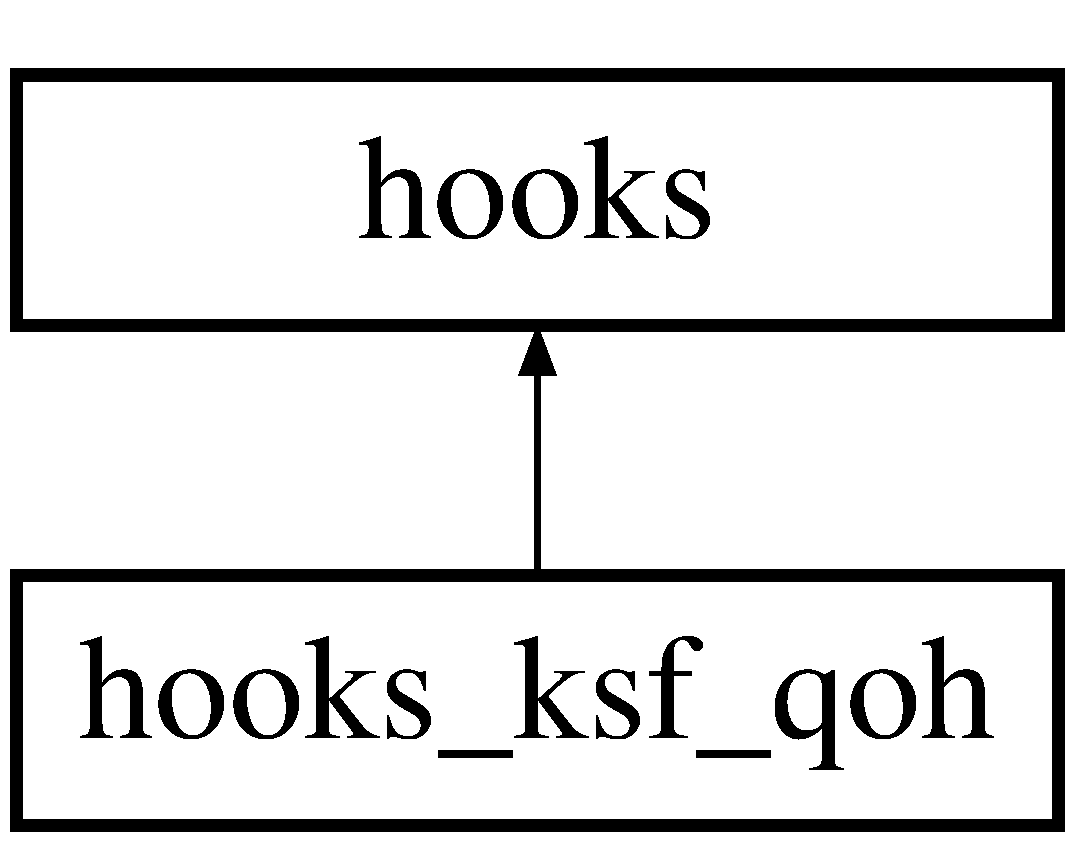
\includegraphics[height=2.000000cm]{d2/d7c/classhooks__ksf__qoh}
\end{center}
\end{figure}
\subsection*{Public Member Functions}
\begin{DoxyCompactItemize}
\item 
\hypertarget{classhooks__ksf__qoh_a9475e2af0e60043a95fc7c93feadc5db}{}\label{classhooks__ksf__qoh_a9475e2af0e60043a95fc7c93feadc5db} 
{\bfseries install\+\_\+options} (\$app)
\item 
\hypertarget{classhooks__ksf__qoh_a16ce6d9c67a774ad4ecf7cecdee5c9b3}{}\label{classhooks__ksf__qoh_a16ce6d9c67a774ad4ecf7cecdee5c9b3} 
{\bfseries install\+\_\+access} ()
\end{DoxyCompactItemize}
\subsection*{Public Attributes}
\begin{DoxyCompactItemize}
\item 
\hypertarget{classhooks__ksf__qoh_aae877d79842f44f3bada169a70f181fa}{}\label{classhooks__ksf__qoh_aae877d79842f44f3bada169a70f181fa} 
{\bfseries \$module\+\_\+name} = \textquotesingle{}Quantity on Hand\textquotesingle{}
\end{DoxyCompactItemize}


The documentation for this class was generated from the following file\+:\begin{DoxyCompactItemize}
\item 
hooks.\+php\end{DoxyCompactItemize}

\hypertarget{classksf__qoh}{}\section{ksf\+\_\+qoh Class Reference}
\label{classksf__qoh}\index{ksf\+\_\+qoh@{ksf\+\_\+qoh}}
Inheritance diagram for ksf\+\_\+qoh\+:\begin{figure}[H]
\begin{center}
\leavevmode
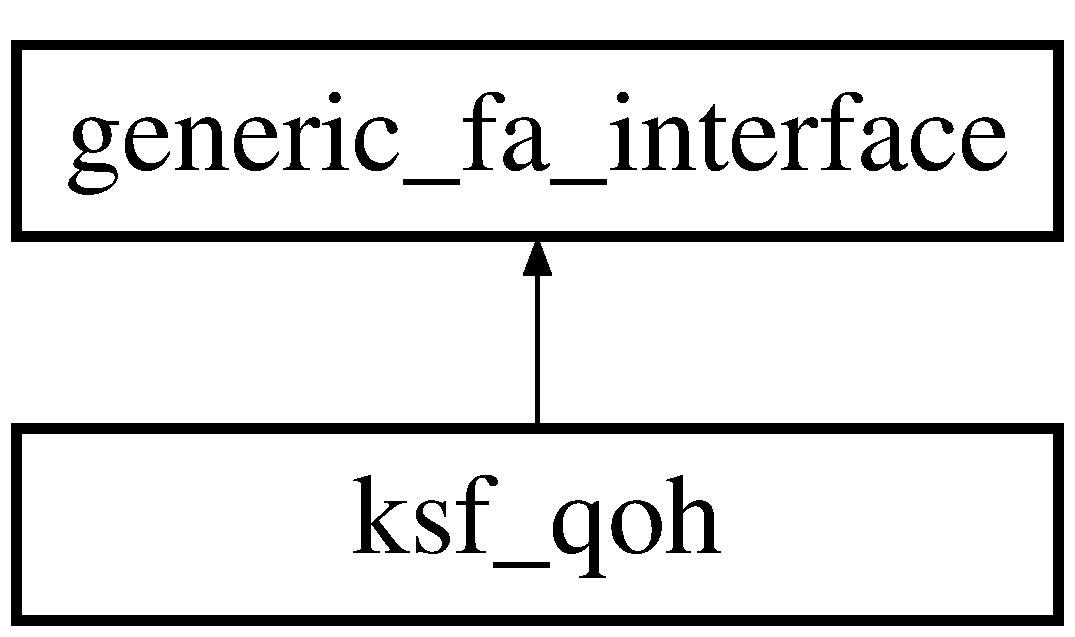
\includegraphics[height=2.000000cm]{d4/ddb/classksf__qoh}
\end{center}
\end{figure}
\subsection*{Public Member Functions}
\begin{DoxyCompactItemize}
\item 
\hypertarget{classksf__qoh_a88b17299dbe9629f0324c9467acb519c}{}\label{classksf__qoh_a88b17299dbe9629f0324c9467acb519c} 
{\bfseries \+\_\+\+\_\+construct} (\$pref\+\_\+tablename)
\item 
\hypertarget{classksf__qoh_a27b8ae75d4ab4242fa873d700844fefc}{}\label{classksf__qoh_a27b8ae75d4ab4242fa873d700844fefc} 
{\bfseries action\+\_\+show\+\_\+form} ()
\item 
\hypertarget{classksf__qoh_a49694928ddf8ba4fb2af958462844adc}{}\label{classksf__qoh_a49694928ddf8ba4fb2af958462844adc} 
{\bfseries install} ()
\item 
\hypertarget{classksf__qoh_ad3d78d238db357e68ec01a8658541863}{}\label{classksf__qoh_ad3d78d238db357e68ec01a8658541863} 
{\bfseries define\+\_\+table} ()
\item 
\hypertarget{classksf__qoh_af8be3379eb49d26640cac2a28e44492e}{}\label{classksf__qoh_af8be3379eb49d26640cac2a28e44492e} 
{\bfseries form\+\_\+\+Q\+OH} ()
\item 
\hypertarget{classksf__qoh_a3ed511b20a8bfa1779fd88811db1487c}{}\label{classksf__qoh_a3ed511b20a8bfa1779fd88811db1487c} 
{\bfseries form\+\_\+\+Q\+O\+H\+\_\+completed} ()
\end{DoxyCompactItemize}
\subsection*{Public Attributes}
\begin{DoxyCompactItemize}
\item 
\hypertarget{classksf__qoh_a46e393cfb2996da9b7d8ab1bae9bec02}{}\label{classksf__qoh_a46e393cfb2996da9b7d8ab1bae9bec02} 
{\bfseries \$lastoid}
\item 
\hypertarget{classksf__qoh_a584caab866fce5180de1dc88dae8bbe0}{}\label{classksf__qoh_a584caab866fce5180de1dc88dae8bbe0} 
{\bfseries \$debug}
\item 
\hypertarget{classksf__qoh_adf1dc3ce6f6aee017abfb3a1dd869951}{}\label{classksf__qoh_adf1dc3ce6f6aee017abfb3a1dd869951} 
{\bfseries \$table\+\_\+interface}
\end{DoxyCompactItemize}


The documentation for this class was generated from the following file\+:\begin{DoxyCompactItemize}
\item 
class.\+ksf\+\_\+qoh.\+php\end{DoxyCompactItemize}

%--- End generated contents ---

% Index
\backmatter
\newpage
\phantomsection
\clearemptydoublepage
\addcontentsline{toc}{chapter}{Index}
\printindex

\end{document}
